\section{Open Challenges and Future Directions}
\label{sec:open-challenges}

Section~\ref{sec:critical-analysis} looked backward: what the surveyed
QIEA-for-MOO literature and this survey's own case study already show
to be weak or under-tested. This section looks forward, organized into
four groups -- the two open questions this survey's own analysis raised
without answering, methodological directions for QIEA-MOO as a field,
technical extensions specific to the case-study pipeline, and the
broader trajectory the field appears to be moving toward.

\subsection{Open Questions Raised by This Survey}
\label{sec:open-challenges:raised}

Two specific questions surfaced earlier in this survey without being
resolved, and we restate them here as concrete starting points rather
than let them dissolve into the more general directions below.

First, Section~\ref{sec:taxonomy:application} found the application
domains covered by the surveyed literature split into two disjoint
clusters -- quantum-inspired algorithms applied to classical
combinatorial or engineering problems, and classical (non-quantum-
inspired) algorithms applied to a genuinely quantum problem domain, as
in this survey's own case study -- with no method in the literature
gathered so far combining both: a Q-bit-represented, quantum-inspired
MOEA applied directly to a quantum-computing problem domain such as
circuit optimization or compilation. Concretely, this would mean
encoding a gate sequence itself as a string of Q-bit amplitude pairs,
with rotation-gate (and perhaps entanglement- or interference-inspired)
operators evolving that encoding directly, rather than -- as this
survey's own case study does -- using an ordinary classical chromosome
of gate tuples inside a classical MOEA. Whether such a representation
would offer any advantage over either cluster alone (e.g.\ a more
natural search-space geometry for gate sequences, given that both
objects are already expressed in the language of qubits and rotations)
is, to our knowledge, untested anywhere in the current literature.

Second, Section~\ref{sec:case-study:hypervolume} found that NSGA-III's
Pareto front is not only smaller than NSGA-II's or SMS-EMOA's under a
shared-reference (fair) hypervolume comparison in this project's own
pipeline, but increasingly so as problem size grows. We could state
\emph{that} finding with confidence; we could not state \emph{why}
without further investigation reaching beyond survey scope --
specifically, whether it traces to Deb and Jain's reference-point
niching providing systematically less selection pressure toward a
front's extremes than crowding distance or hypervolume-driven
environmental selection do, as this pipeline's block sizes grow, or to
some interaction specific to this pipeline's block-partitioned setting
that would not generalize to non-partitioned NSGA-III use. Distinguishing
these is exactly the kind of question the separate, forthcoming
empirical results paper is positioned to pursue, since it requires
running controlled ablations this survey does not.

\subsection{Methodological Directions for QIEA-MOO}
\label{sec:open-challenges:methodological}

Several of Section~\ref{sec:critical-analysis:per-category}'s
per-category weaknesses point directly at concrete methodological gaps
rather than only diagnosing a problem. The selection-mechanism
concentration on NSGA-II's crowding distance
(Section~\ref{sec:taxonomy:selection}) is the clearest: no surveyed
method has paired the Q-bit representation with NSGA-III's
reference-point niching, SPEA2's density estimator, MOEA/D's
decomposition, or SMS-EMOA's hypervolume-driven selection, so which of
these pairings would actually work well -- and whether any of them
would shift the operator-versus-selection balance discussed in
Section~\ref{sec:taxonomy:operator} -- is entirely open. Relatedly, a
genuinely interference-based quantum-inspired operator, as opposed to
the rotation-gate-plus-one-bolt-on pattern found throughout the
surveyed literature, has yet to be demonstrated at all. A third
direction is evaluative rather than architectural: establishing a
shared benchmark protocol that compares QIEA-MOO methods against each
other, not only each against NSGA-II in isolation
(Section~\ref{sec:critical-analysis:per-category}), would be a modest
undertaking relative to proposing a new algorithm, but it is precisely
the missing piece that would let the field's many NSGA-II-beating
claims be weighed against one another. Finally, on the representation
side, \citet{weakconstraintpareto2025}'s weak constraint-Pareto
dominance mechanism has no QIEA-MOO application yet and, per
Section~\ref{sec:critical-analysis:per-category}, no immediate purchase
on this survey's own case study either, since its per-block objectives
are soft rather than hard constraints today -- but a future QIEA-MOO
method or pipeline extension that does introduce a hard feasibility
cutoff (e.g.\ a minimum fidelity threshold treated as a constraint
rather than a maximized objective) would have a directly applicable
mechanism waiting for it.

\subsection{Extensions to the Case-Study Pipeline}
\label{sec:open-challenges:pipeline}

A separate set of directions is specific to the quantum-circuit-
optimization side of the case study rather than to QIEA-MOO as a
field, gathered from related work during this survey's own literature
search rather than from the surveyed QIEA-MOO methods themselves.
On the per-block optimizer side
(Section~\ref{sec:case-study:algorithms}), the same
\texttt{BLOCK\_OPTIMIZERS}-style registry that already lets NSGA-II,
NSGA-III, and SMS-EMOA slot in interchangeably could take further
entries: \citet{ulungu1999mosa}'s MOSA is the least costly next
addition, since it extends the pipeline's existing simulated-annealing
injection machinery rather than introducing a new mechanism from
scratch, followed by \citet{zitzler2004ibea}'s IBEA (generalizing
SMS-EMOA's hypervolume-driven idea to other indicators) or a
decomposition-based method in the style of MOEA/D, with SPEA2 -- best
cited today alongside \citet{alghouass2025spea2beatsnsga2}'s stronger,
more recent approximation-guarantee result rather than only the
original 2001 paper (Section~\ref{sec:critical-analysis:per-category})
-- and \citet{coello2002mopso}'s MOPSO, a different paradigm entirely,
as costlier additions requiring a continuous-relaxation or discrete-PSO
adaptation of the pipeline's chromosome encoding. On the objective
side, a noise- or crosstalk-aware term~\citep{hua2022crosstalk} could
become a fourth per-block objective, extending the pipeline's existing
(currently placeholder) crosstalk term in its simulated-annealing
injection energy, though this would require a noise model the pipeline
does not yet have. On scalability specifically, the pipeline's fidelity
estimation already required substantial, family-specific engineering to
reach the qubit counts used in Section~\ref{sec:case-study:pipeline}.
Figure~\ref{fig:scaling-wallclock} shows why this remains an open cost
rather than a solved one: total wall-clock time grows sharply with
qubit count for four of the five circuit families -- most steeply for
\texttt{hw\_efficient\_ansatz} (roughly 22s at $n{=}8$ to over 1{,}000s
at $n{=}20$) and \texttt{qft}, more gently for \texttt{weak\_random} --
while \texttt{qaoa\_maxcut} is non-monotonic (26s, 75s, 43s at $n{=}8$,
$12$, and its own $n{=}16$ ceiling respectively), plausibly an artifact
of the statevector-backend fidelity settings that
Section~\ref{sec:case-study:pipeline} notes are applied per family
above certain thresholds rather than a genuine efficiency gain at
larger $n$ -- a wrinkle we did not investigate further here.
Classical-shadow or tensor-network fidelity
estimation~\citep{fu2022shadow} is a concrete candidate for pushing
past where the current echo-test and statevector Monte-Carlo backends
become memory- or time-bound.

\begin{figure}[htbp]
  \centering
  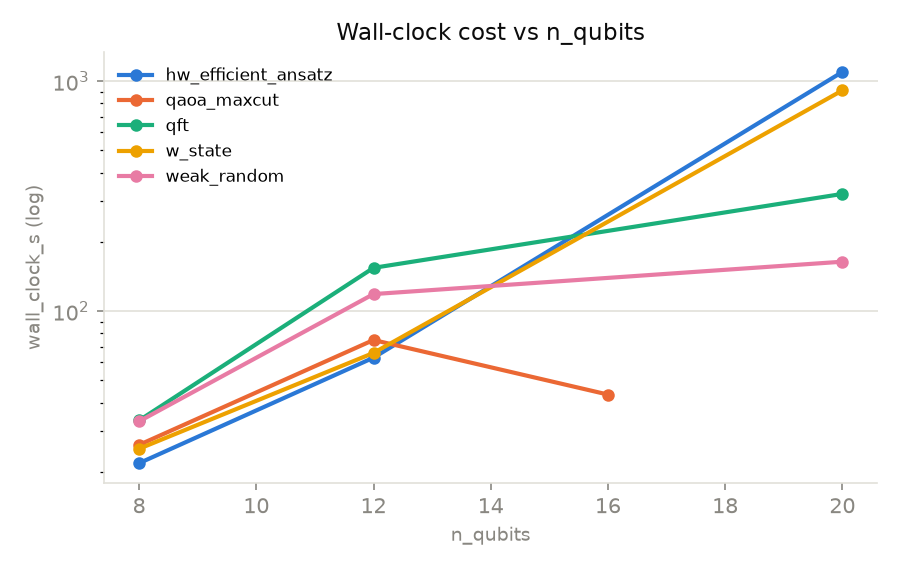
\includegraphics[width=0.75\linewidth]{figures/scaling_wallclock.png}
  \caption{Total wall-clock cost vs.\ qubit count, per circuit family,
    pooled across the three per-block optimizers of the 225-run core
    baseline (log-scaled $y$-axis). Four families grow sharply with
    $n$; \texttt{qaoa\_maxcut}'s three-point trend is not monotonic
    (see discussion above).}
  \label{fig:scaling-wallclock}
\end{figure}

Finally, two structural extensions target
stages this survey's taxonomy does not otherwise cover: reinforcement
learning combined with ZX-calculus~\citep{riu2023rlzx} as an
alternative to the pipeline's hand-rolled compression passes, and
hyperedge-aware partitioning~\citep{sweeney2025hypergraph} in place of
the fixed-modularity Louvain partitioning
Section~\ref{sec:case-study:pipeline} describes. None of these is
implemented in the pipeline today; each is a scoped, independently
addable extension rather than a redesign.

\subsection{Where the Field Appears to Be Heading}
\label{sec:open-challenges:trajectory}

Beyond specific gaps, two recent surveys outside the QIEA-MOO
literature proper suggest where multi-objective optimization as a
whole is heading, for context rather than as a near-term target for
either QIEA-MOO or this survey's case study.
\citet{li2015manyobjective}'s many-objective survey's seven-class
taxonomy (relaxed-dominance, diversity-based, aggregation-based,
indicator-based, reference-set-based, preference-based, and
dimensionality-reduction methods) is a reminder that this survey's own
five classical baselines (Section~\ref{sec:background:moea}) sample
only some of that landscape, and a QIEA-MOO method built around
preference articulation or dimensionality reduction, rather than any of
the five selection paradigms named in
Section~\ref{sec:taxonomy:selection}, remains unexplored.
\citet{doerr2026paretoneural}'s more recent five-level taxonomy --
classical MOEA, ML-guided, RL-driven, LLM-driven, and hybrid
neuro-evolutionary methods -- places every method surveyed in this
paper, and this survey's own case study, at its first level; the field
this taxonomy describes is moving toward learned and neural surrogate
models and RL- or LLM-guided search rather than purely evolutionary
operators, a considerably larger architectural departure than any
single direction in Sections~\ref{sec:open-challenges:methodological}
or~\ref{sec:open-challenges:pipeline} above. We do not read this as a
reason to treat QIEA-MOO or block-partitioned quantum circuit
optimization as obsolete -- both remain useful, interpretable,
comparatively cheap-to-run methods exactly where a learned surrogate's
training cost or data requirement is not justified -- but a
QIEA-MOO method that hybridizes a Q-bit representation with a learned
selection or variation mechanism, rather than only with the classical
selection paradigms surveyed in
Section~\ref{sec:taxonomy:hybridization}, is a direction no method
gathered for this survey has yet taken. Finally,
\citet{zheng2025weakparetoboundary}'s structural critique of
Pareto-dominance-based EMO (Section~\ref{sec:critical-analysis:cross-cutting})
is itself forward-looking as much as critical: a next generation of
QIEA-MOO methods, and of this survey's own case-study pipeline, that
addressed the weak Pareto boundary directly -- rather than continuing to
build on the dominance relation as-is -- would be responding to a
weakness identified in the same year as this survey, not one already
absorbed into current practice.
